\documentclass[11pt]{beamer}
\usepackage[utf8]{inputenc}
\usepackage[T1]{fontenc}
\usetheme{default}
\begin{document}
	\author{Jacob Nieswand}
	\title{Zsfg Masterarbeit}
	%\subtitle{}
	%\logo{}
	%\institute{}
	%\date{}
	%\subject{}
	%\setbeamercovered{transparent}
	%\setbeamertemplate{navigation symbols}{}
	\begin{frame}[plain]
	\maketitle
\end{frame}

\begin{frame}
\frametitle{Light Field Parametrization}
\begin{figure}[h]
	\centering
	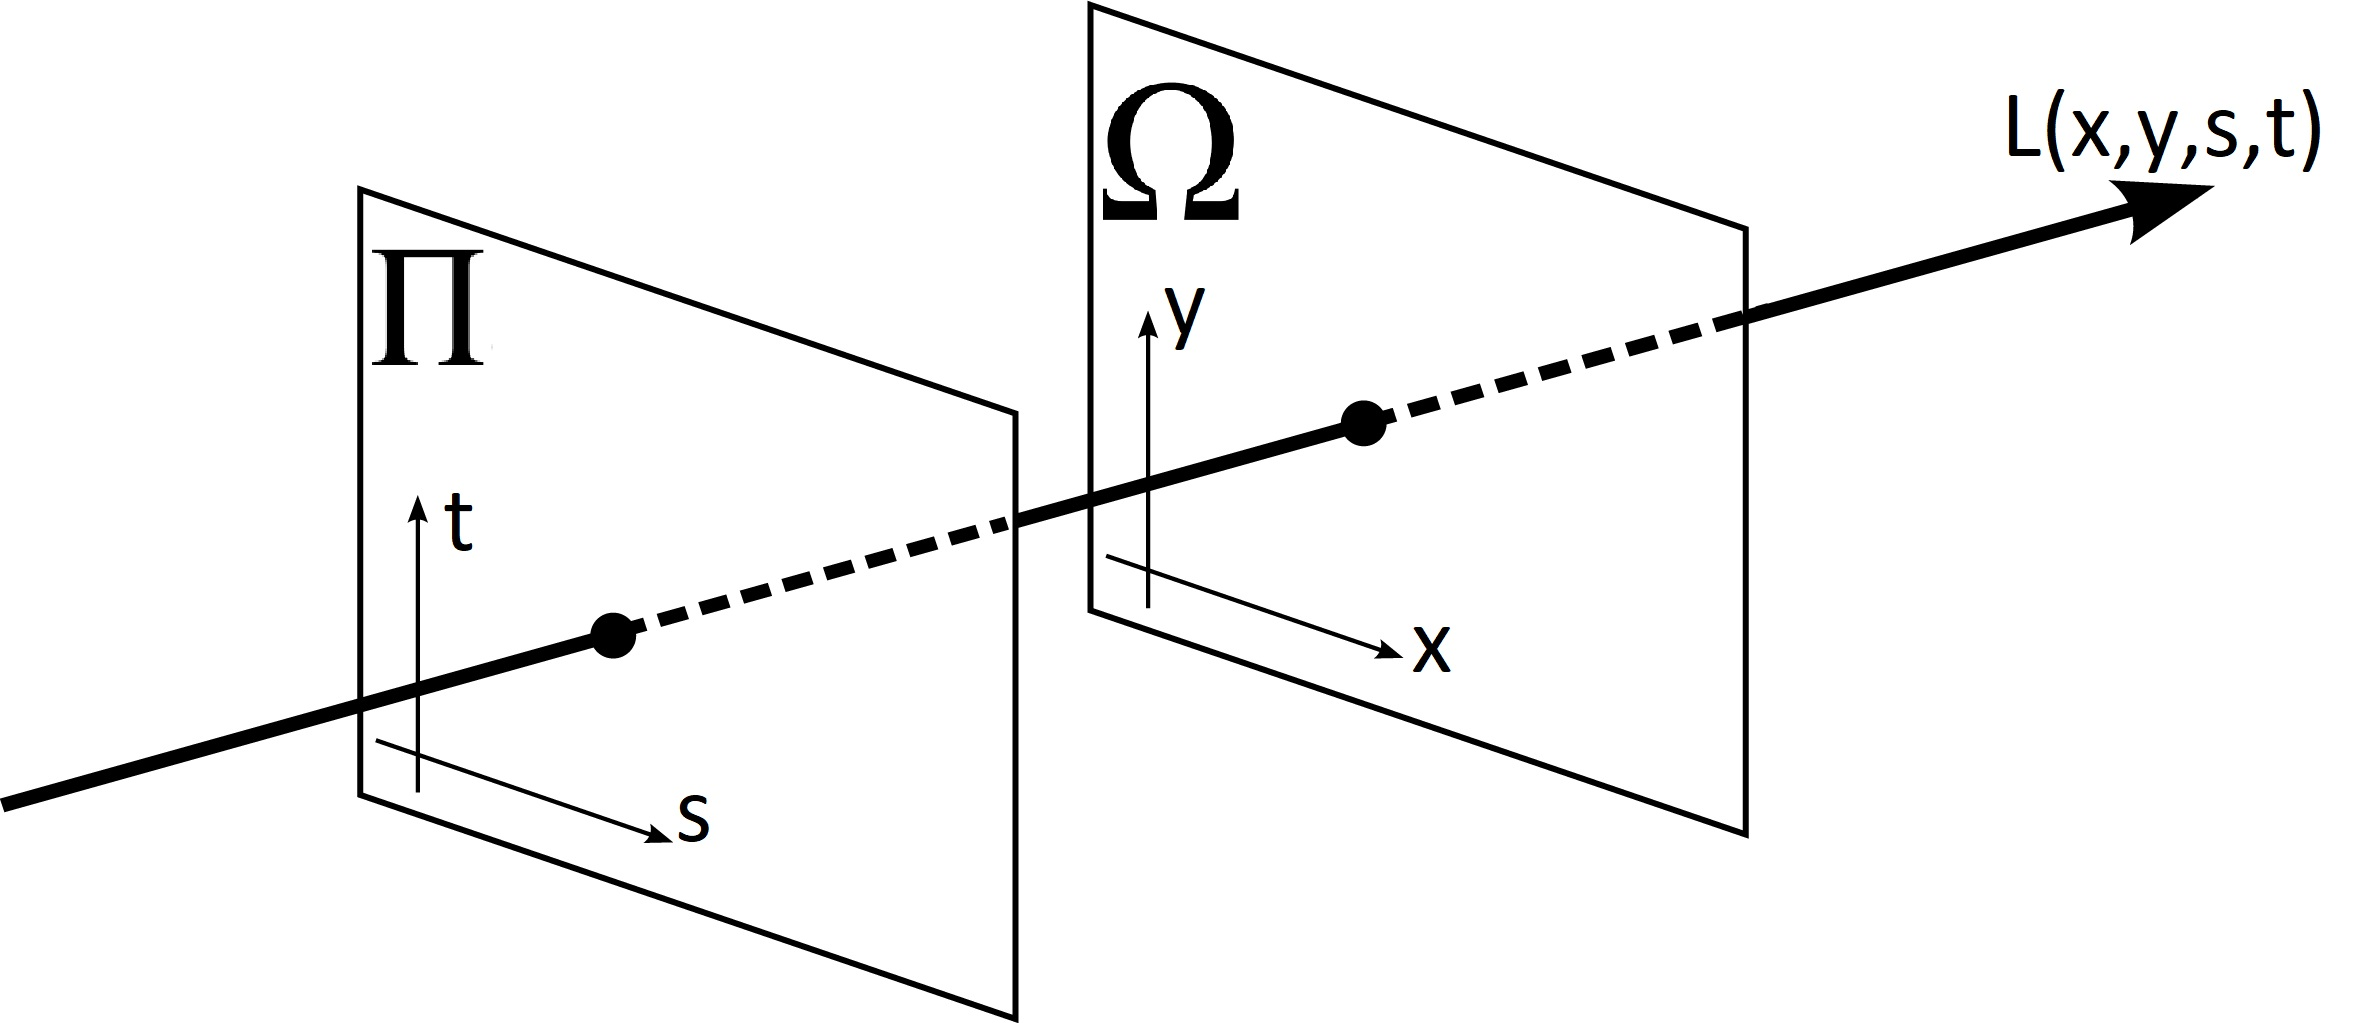
\includegraphics[width=0.7\linewidth]{images/twoplane_param}
	\caption[Two-plane parametrisation]{In a 4-dimensional two-plane parametrisation a light ray is characterized by the intersection with two parallel planes. we refer to the plane  $\Pi$ as the camera plane and the plane $\Omega$ as the image plane.}
	\label{fig:twoplaneparam}
\end{figure}
\end{frame}
 \begin{frame}
 	\frametitle{Epipolar Plane Images}
 	\begin{figure}
 		\centering
 		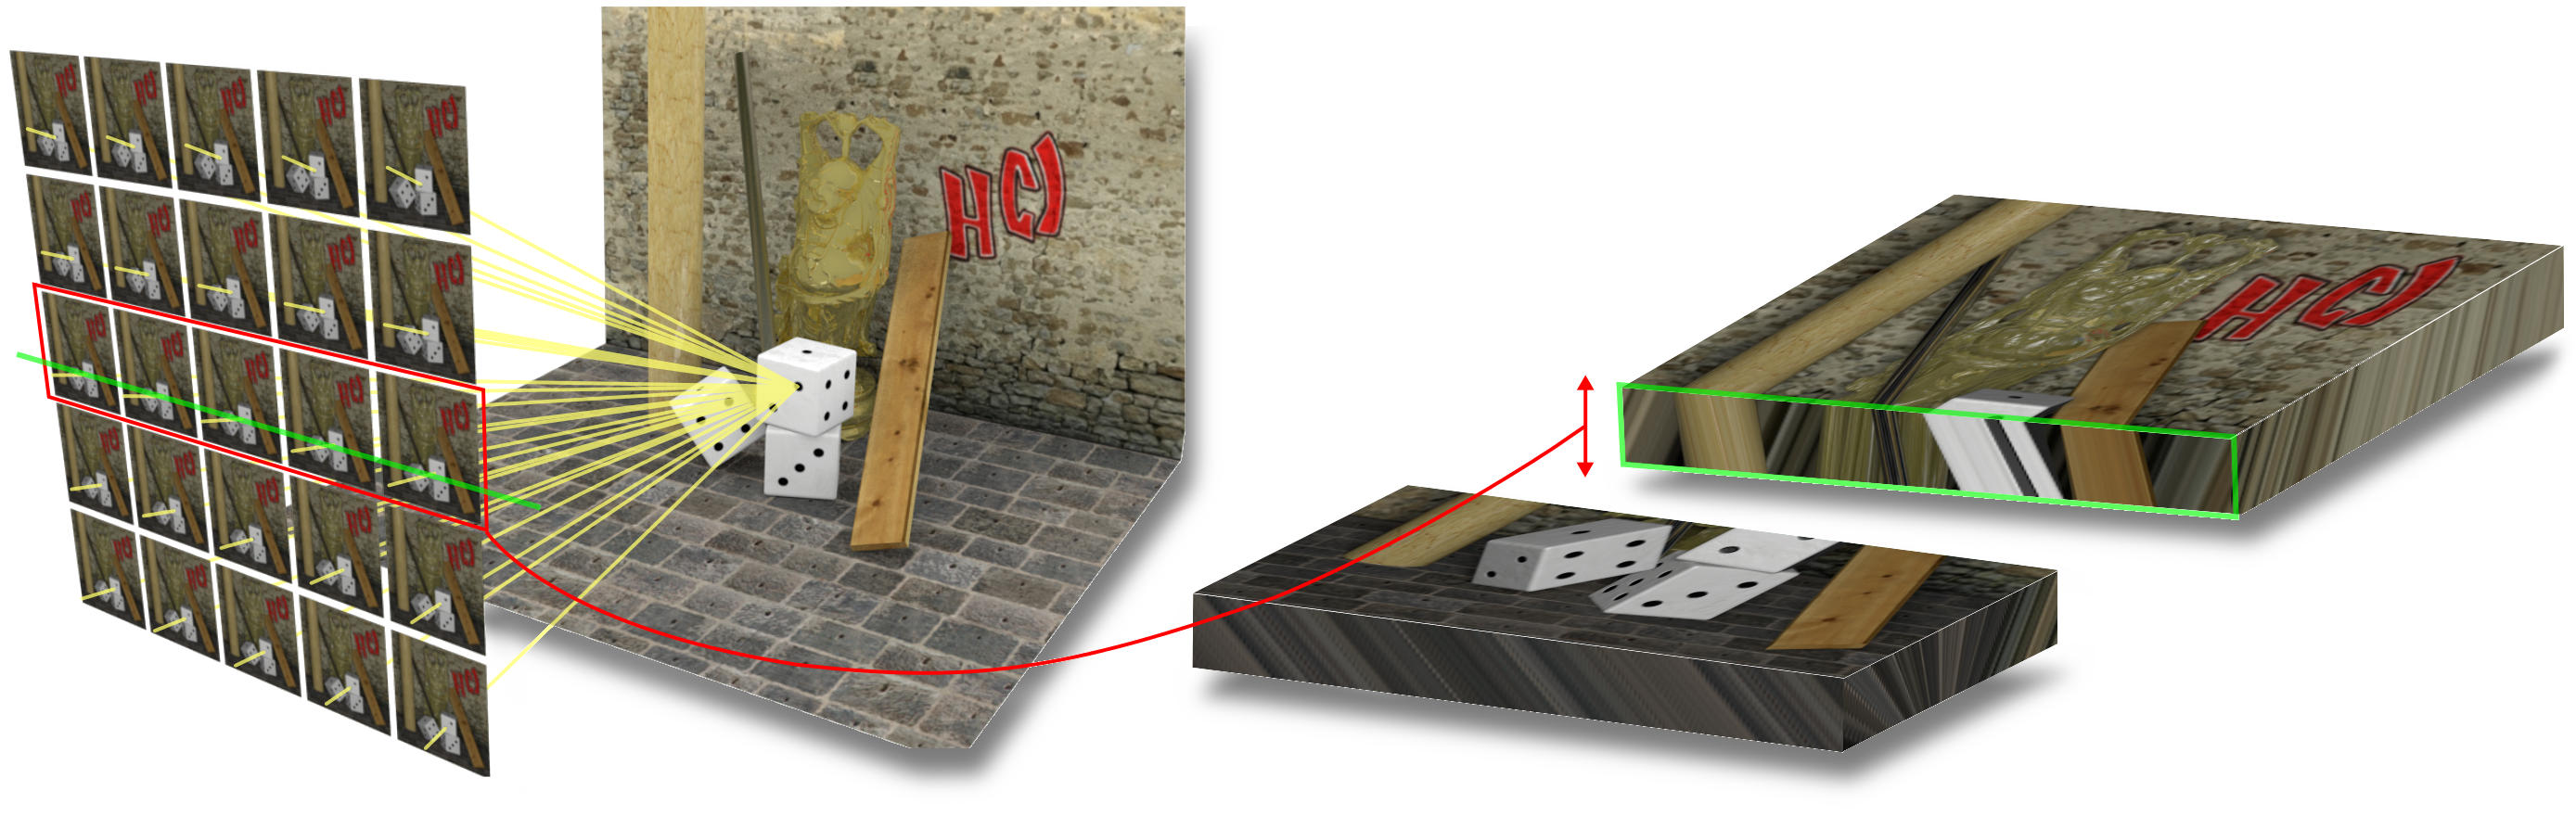
\includegraphics[width=1\linewidth]{images/epiVisualization}
 		\caption[Visualization of an EPI extraction]{Visualization of an Epipolar Plane Image extractoin: A camera array takes images of the same scene from slightly different angles (left array). For a fixed image coordinate $y^*$ (green) and a fixed camera coordinate $t^*$ (red) the pixels are extracted and stacked up resulting in an EPI $\Sigma_{y^*, t^*}$ (green box on the right).}
 		\label{fig:epivisualization}
 	\end{figure}
 	
 \end{frame}
\begin{frame}
	\frametitle{EPI}
	\begin{figure}
		\centering
		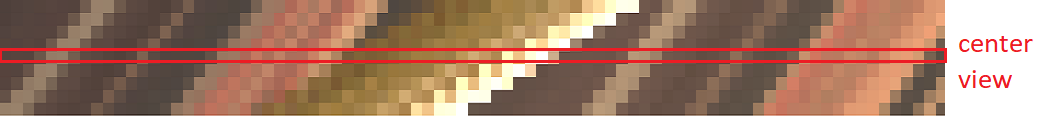
\includegraphics[width=1\linewidth]{images/simple_epi}
		\caption[Example Epipolar Plane image]{An Epipolar Plane Image (EPI) that consists of 9 rows (9 equidistant views or sample points in the camera plane). Points with the same color correspond to the same scene point. Since the viewpoints are slightly shifted, the scene point is also shifted in each view by the disparity $d$. Marked in red one can identify the center position of the camera viewpoints.}
		\label{fig:simpleepi}
	\end{figure}
\end{frame}
\begin{frame}
\frametitle{Refocussing an EPI}
\begin{figure}
	\centering
	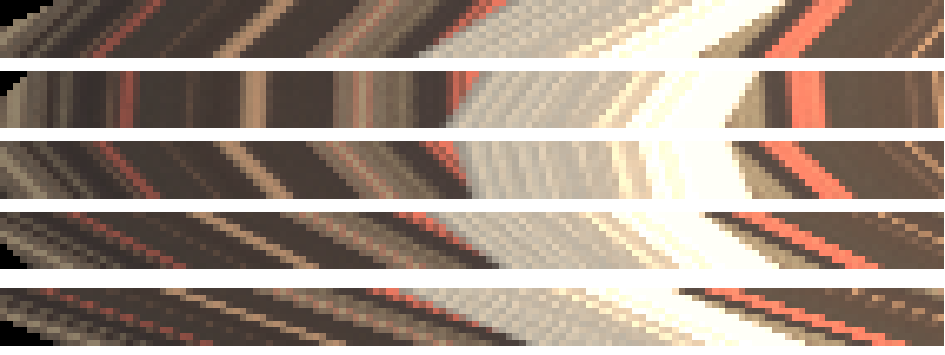
\includegraphics[width=0.7\linewidth]{images/refocused_cut}
	\caption[Refocussed EPI]{The EPI is refocussed by integer disparity steps. If the slope at a scene point is zero (vertical line) the EPI is perfectly focussed on that point. An integration of all views would still result in a sharp image at the corresponding depth.}
	\label{fig:refocusedcut}
\end{figure}
\end{frame}

\begin{frame}
\frametitle{Occlusion Problem}
\begin{figure}
	\centering
	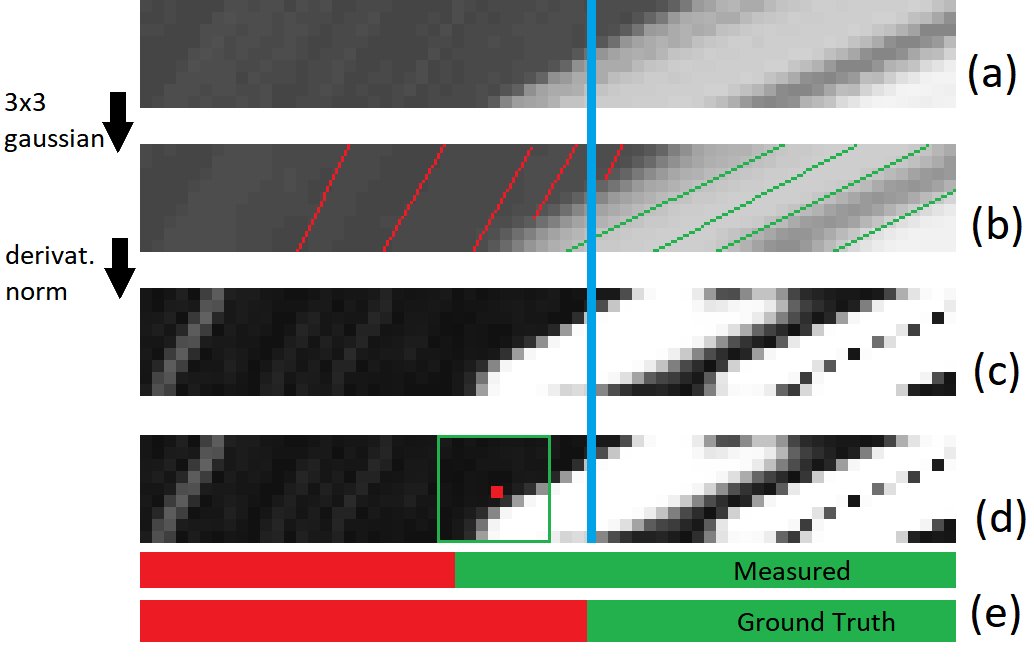
\includegraphics[width=0.7\linewidth]{images/occlusion_painted2}
	\caption[Occlusion in an EPI]{(a) The structure of an occlusion border in a gray-value EPI. (b) Before calculating the gradient, the EPI is smoothed with a $3 \times 3$ gaussian kernel. One sees the smoothed EPI with colored lines indicating the Ground Truth orientation. (c) shows the norm of the gradient calculated via the Scharr-filter. White significates a high gradient, black significates low gradient. In (d) the local environment around the red dot $(x_r,y_r)$ as an example point is marked to show which gradient values go into the structure tensor components $J(x_r,y_r)$. (e) marks the orientation labeling measured and ground truth. The blue line marks the transition in the center view that corresponds with the ground thruth labeling. }
	\label{fig:occlusion}
\end{figure}
\end{frame}

\begin{frame}
\frametitle{Sandclock kernel}
\begin{figure}
	\centering
	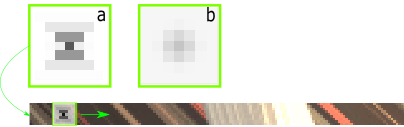
\includegraphics[width=0.7\linewidth]{images/sandclock.png}
	\caption[Sandclock Kernel]{(a) shows a custom-shaped kernel in form of a sandclock. (b) shows a normal gaussian kernel.}
	\label{fig:sandclock}
\end{figure}
\end{frame}

\begin{frame}
\frametitle{Bilateral filtering}
\begin{figure}
	\centering
	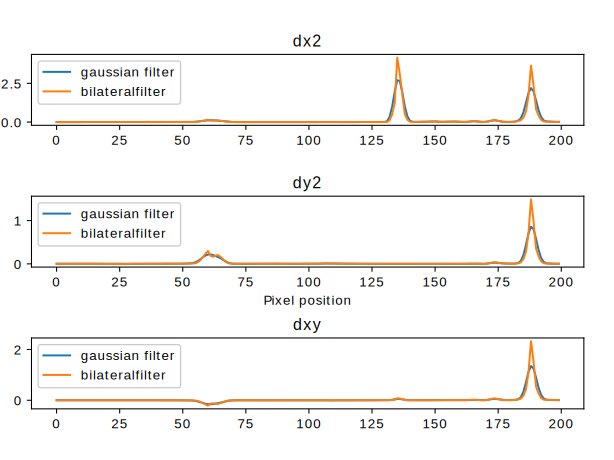
\includegraphics[width=0.7\linewidth]{images/bilat}
	\caption[Bilateral filtering]{Bilateral filtering of an epi}
	\label{fig:bilat}
\end{figure}
\end{frame}

\begin{frame}
\frametitle{Thresholding Gradients}
\begin{align}
\tilde{\vec \nabla}(x,y) &= \begin{cases}
\frac{\text{threshold}}{\text{norm}} \vec \nabla(x,y) \quad &\text{if}\quad \text{norm}> \text{threshold}\\
\tilde{\vec \nabla}(x,y)\qquad &\text{else}\\
\end{cases} \\
\text{with} \quad \text{norm} &= \sqrt{\nabla_x(x,y)^2 + \nabla_y(x,y)^2}.\\
\end{align}
\end{frame}

\begin{frame}
\frametitle{Occlusion Segmentation}
\begin{enumerate}
	\item Segmentate the transitions and the rest of the EPI with a binary mask.
	\item Calculate the structure tensor components on the masked gradient of the EPI. All masked gradients are zero and do not affect the local environment structure.
	\item Calculate the structure tensor components again, now on the inverted masked gradient of the EPI.
\end{enumerate}
\end{frame}

\begin{frame}
\frametitle{Occlusion Segmentation}
\begin{figure}
	\centering
	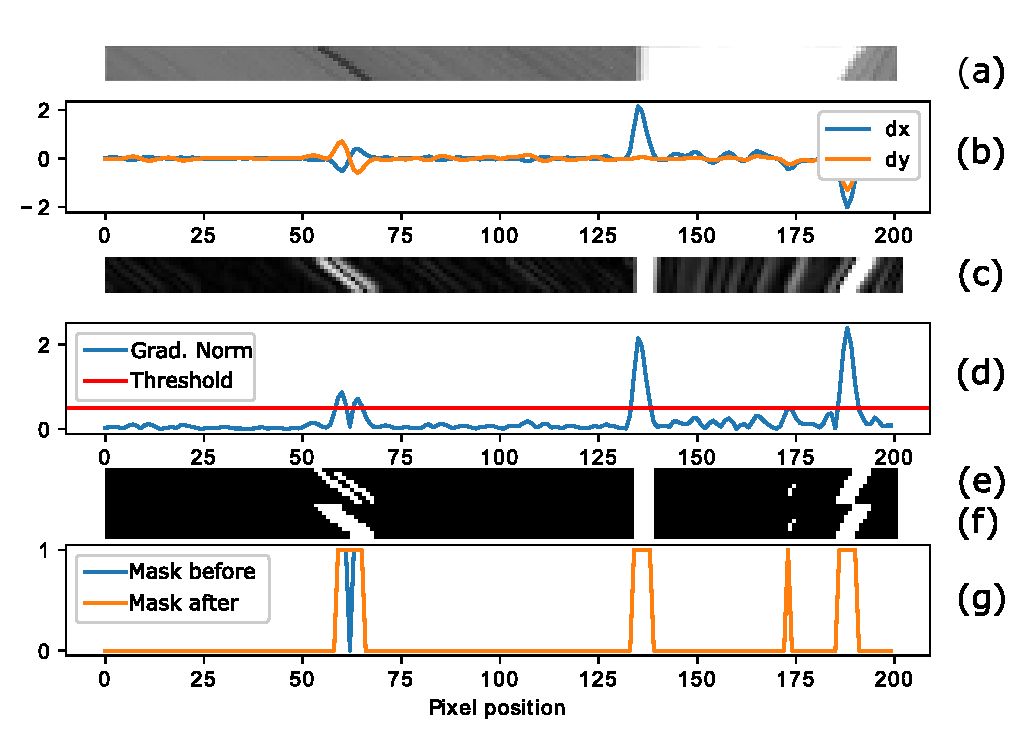
\includegraphics[width=1\linewidth]{images/derivatives_full}
	\caption[Segmentating an EPI]{(a) Input EPI to be segmented. (b) show the local derivatives along the center view line. (c) shows the vector norm of the derivative. (d) shows the center view norm with the threshold that is applyed to mask transitions. (e) shows the resulting mask. (f) shows the improved mask using morphological image processing. (g) shows the mask at the center view before and after using morph. image processing. }
	\label{fig:derivativesfull}
	
\end{figure}
\end{frame}

\begin{frame}
\frametitle{Morphological Closing}
\begin{figure}
	\centering
	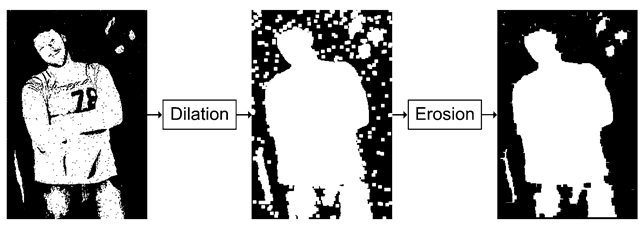
\includegraphics[width=0.7\linewidth]{images/closing}
	\caption[Morphological closing]{Morphological closing is a combination of Dilation and Erosion. Dilation uses a custom-sized kernel and turnes any 0 to 1, if at least one 1 isfound in the local environment. Erosion turnes any 1 to 0, if at least one 0 is found in the local environment.}
	\label{fig:closing}
\end{figure}
\end{frame}

\begin{frame}
\frametitle{Alternative to coherence}
\begin{equation}\label{eq:disparity2}
d = \tan\left(\frac{1}{2} \arctan\left( \frac{J_{22}-J_{11}}{2J_{12}}\right)\right),
\end{equation}
\begin{equation}\label{eq:err_d}
\Delta d = \sqrt{\left(\frac{\partial d}{J_{11}}  \Delta J_{11}\right)^2 + \left(\frac{\partial d}{J_{22}}  \Delta J_{22}\right)^2 + \left(\frac{\partial d}{J_{12}} \Delta J_{12}\right)^2 }
\end{equation}
\begin{equation}\label{eq:deviation_d}
\Delta d =\sqrt{\left(\frac{0.5\cdot(d^2+1)}{x^2+1}\cdot x\right)^2 \cdot \left(\left|\frac{\Delta J_{12}}{J_{12}}\right|^2 + \left|\frac{\Delta J_{11}}{J_{11}-J_{22}}\right|^2 + \left|\frac{\Delta J_{22}}{J_{11}-J_{22}}\right|^2\right)}
\end{equation}
 \begin{align}\label{eq:std_struct}
\Delta J_{11} &= G *|2\nabla_x|\Delta\nabla_x\\
\Delta J_{22} &= G *|2\nabla_y|\Delta\nabla_y\\
\Delta J_{12} &= G *\sqrt{\nabla_x^2\Delta\nabla_y^2 + \nabla_y^2\Delta\nabla_x^2}
\end{align}
\end{frame}

\begin{frame}
\frametitle{Alternative to coherence}
\begin{align}\label{eq:normed_std}
\Delta\nabla_{x, \text{normalized}} &= \sqrt{E[\nabla_{x, \text{normalized}}^2] - E[\nabla_{x, \text{normalized}}]^2}\\
\Delta\nabla_{y, \text{normalized}} &= \sqrt{E[\nabla_{y, \text{normalized}}^2] - E[\nabla_{y, \text{normalized}}]^2}
\end{align}
The interrelation between $\Delta\nabla_{y, \text{normalized}}$ and  $\Delta\nabla_x$ is given by
\begin{align}\label{eq:norm_error}
\nabla_{x, \text{normalized}} &= \frac{1}{\sqrt{\nabla_x^2 + \nabla_y^2}}\nabla_x \\
\Delta \nabla_{x, \text{normalized}} &\approx  \frac{1}{\sqrt{\nabla_x^2 + \nabla_y^2}}\Delta\nabla_x,
\end{align}
\end{frame}

\begin{frame}
\frametitle{Alternative to Coherence}
\begin{align}\label{eq:normed_std_final}
\Delta\nabla_{x} &=  \sqrt{\nabla_x^2 + \nabla_y^2} \cdot \sqrt{E[\nabla_{x, \text{normalized}}^2] - E[\nabla_{x, \text{normalized}}]^2}\\
\Delta\nabla_{y} &= \sqrt{\nabla_x^2 + \nabla_y^2} \cdot \sqrt{E[\nabla_{y, \text{normalized}}^2] - E[\nabla_{y, \text{normalized}}]^2},
\end{align}
\end{frame}



\begin{frame}
\frametitle{SemiGLobal Matching}
\begin{equation}\label{eq:global_sgm_cont}
E(d) = \sum_{\vec p} \left(C(\vec{p}, d_{\vec p}) + \sum_{q\in N_p} 
\begin{cases}
P1\cdot |d_{\vec p} - d_{\vec q}|  & \text{ if }|d_{\vec p} - d_{\vec q}| \leq 1\\
P2 & \text{ if }|d_{\vec p} - d_{\vec q}| > 1\\
\end{cases}  
\right).
\end{equation}
\begin{figure}
	\centering
	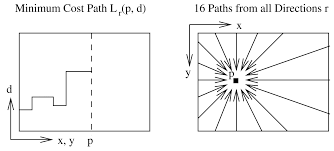
\includegraphics[width=0.7\linewidth]{images/sgm_paths}
	\caption[Discrete scanline to continuous scanline]{Scanlines give exact solution for 1-D minimize problem.}
	\label{fig:discretecont}
\end{figure}

\end{frame}

\begin{frame}
\frametitle{SemiGLobal Matching}
\begin{equation}\label{key}
P2' =  \frac{P2}{\sqrt{(Im_b^2 +Im_r^2 + Im_g^2)}},
\end{equation}
For ST-pipeline:
\begin{equation}\label{eq:global_sgm_cont_occlusion}
E(d) = \sum_{\vec p} \left(C(\vec{p}, d_{\vec p}) + \sum_{q\in N_p} 
\begin{cases}
P1\cdot |d_{\vec p} - d_{\vec q}|  & \text{ if }|d_{\vec p} - d_{\vec q}| \leq 1\\
P2 & \text{ if }d_{\vec p} - d_{\vec q} > 1\\
P3 & \text{ if }d_{\vec p} - d_{\vec q} < -1\\
\end{cases}  
\right).
\end{equation}
\end{frame}

\begin{frame}
\frametitle{Evaluation: Depth-from-focus}
	\begin{figure}
	\centering
	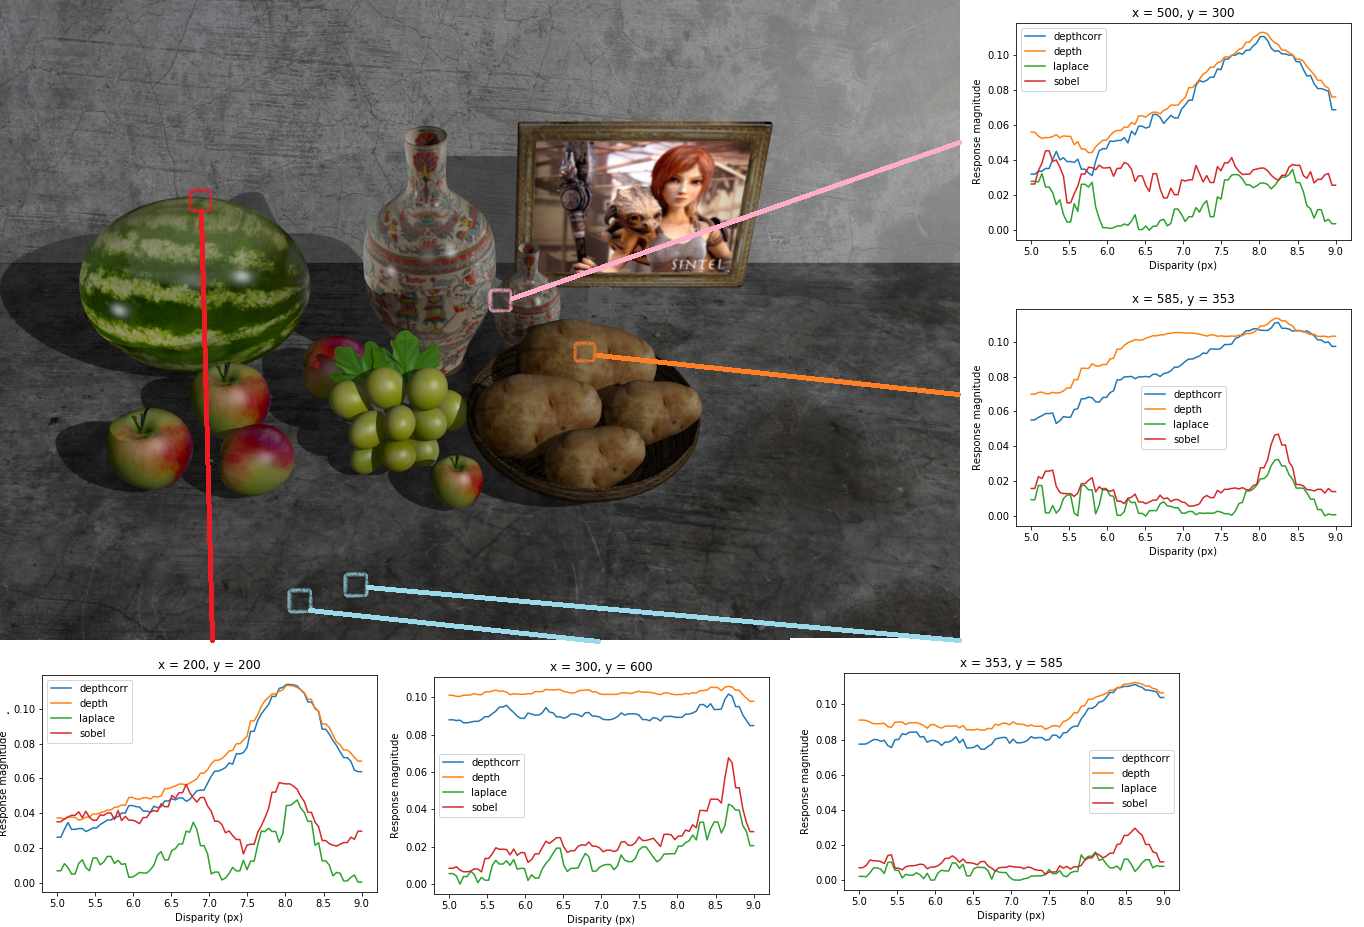
\includegraphics[width=1\linewidth]{images/original_marked}
	\label{fig:originalmarked}
\end{figure}
\end{frame}

\begin{frame}
\frametitle{Evaluation: Depth-from-focus}
\begin{figure}
	\centering
	\includegraphics[width=0.9\linewidth]{images/result_depth_from_focus_res20}
	\caption[Depth from focus: depthmaps]{The depth maps of the scenes (from up to down) \textit{complextestscene, cotton, occlusiontestscene, pens, testscene, tiltplane} is depicted for different depth-from-focus techniques. The Disparity stepsize is 1/20.}
	\label{fig:resultdepthfromfocus}
\end{figure}
\end{frame}

\begin{frame}
\frametitle{Evaluation:Sandclock kernel}
\begin{figure}
	\centering
	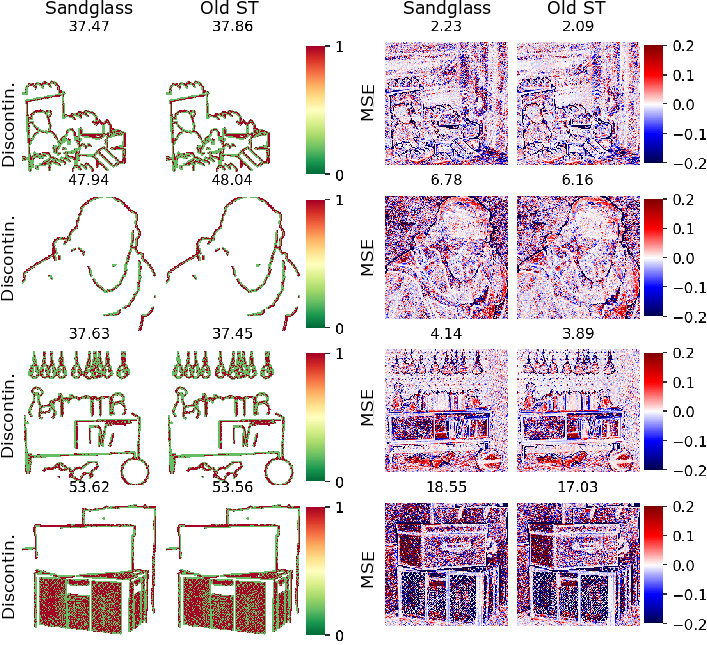
\includegraphics[width=0.7\linewidth]{images/sandclock_results}
	\caption[Results with custom sized kernel]{Comparison between the normal structure tensor and the sandclock- like kernel for the scenes \textit{dino, cotton, sideboard, boxes}. The left side compares the mean squared errors in the disparity map, the right side shows the error where discontinuities in the disparity map are masked explicitely.}
	\label{fig:sandclockresults}
\end{figure}
\end{frame}

\begin{frame}
\frametitle{Evaluation: Bilateral filtering}
\begin{figure}
	\centering
	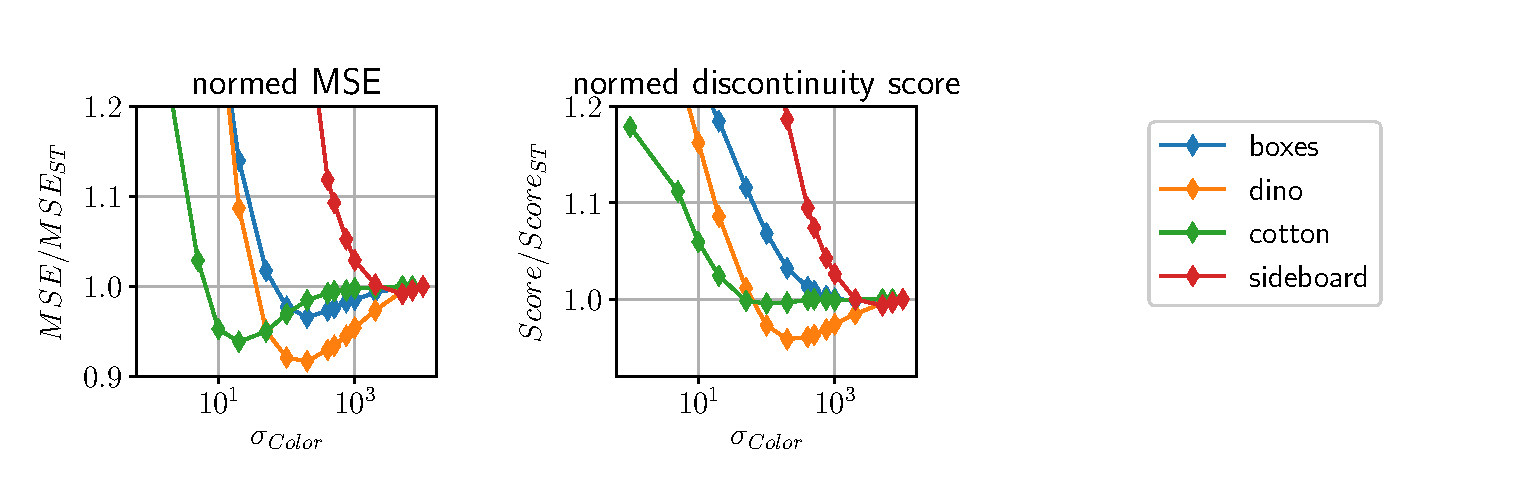
\includegraphics[width=0.7\linewidth]{images/bilateral_norm_params}
	\caption[Parameter dependency for bilateral filtering]{Bilateral filtering with Structure Tensor Components themselves as the guide:On the left the Mean Squared error for different scenes in function of the $\sigma_\text{Color}$ of the bilateral filtering is shown, devided by the MSE with using a gaussian filter. On the right the Discontinuity score based on \cite{honauer2016benchmark} is shown, also normed to the Score using the standard gaussian filter.}
	\label{fig:bilateralnormparams}
\end{figure}
\end{frame}

\begin{frame}
\frametitle{Evaluation: Bilateral filtering}
\begin{figure}
	\centering
	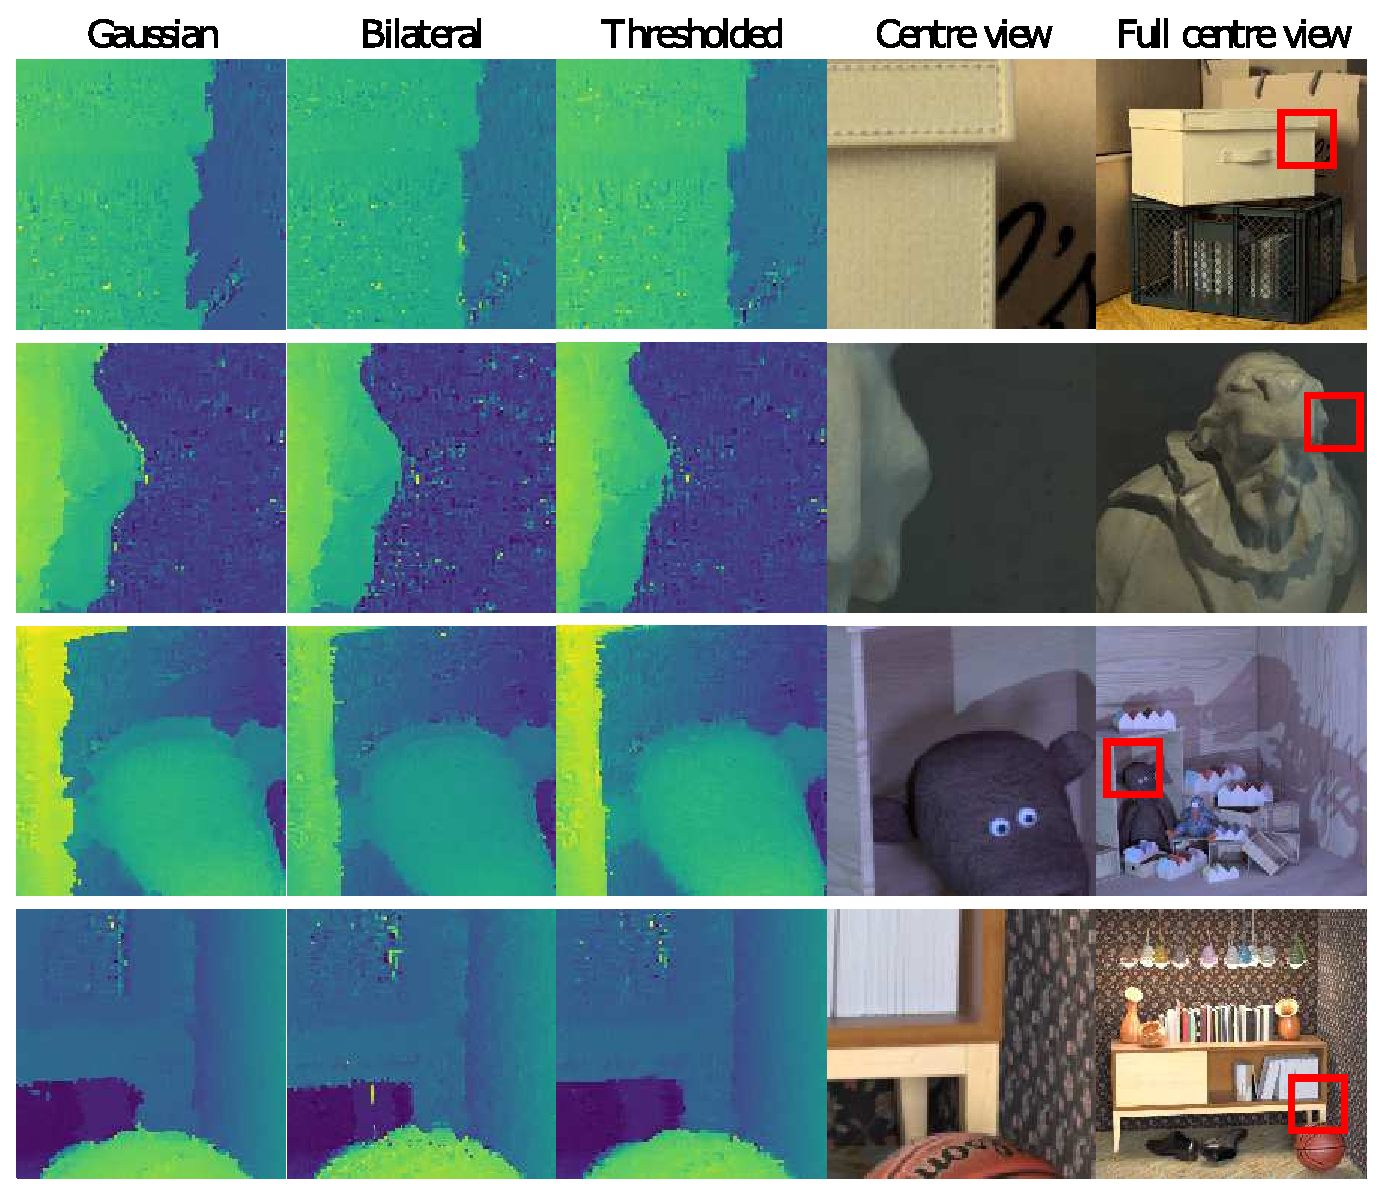
\includegraphics[width=0.9\linewidth]{images/thresh_results}
	\caption[Disparity map Zoom-ins for different methods]{Disparity map Zoom-ins for different Structure Tensor filtering. From Left to right gaussian filtering, bilateral filtering and gaussian filtering when thresholding the gradients.}
	\label{fig:threshresults}
\end{figure}
\end{frame}

\begin{frame}
\frametitle{Evaluation: Thresholding gradients}
\begin{figure}
	\centering
	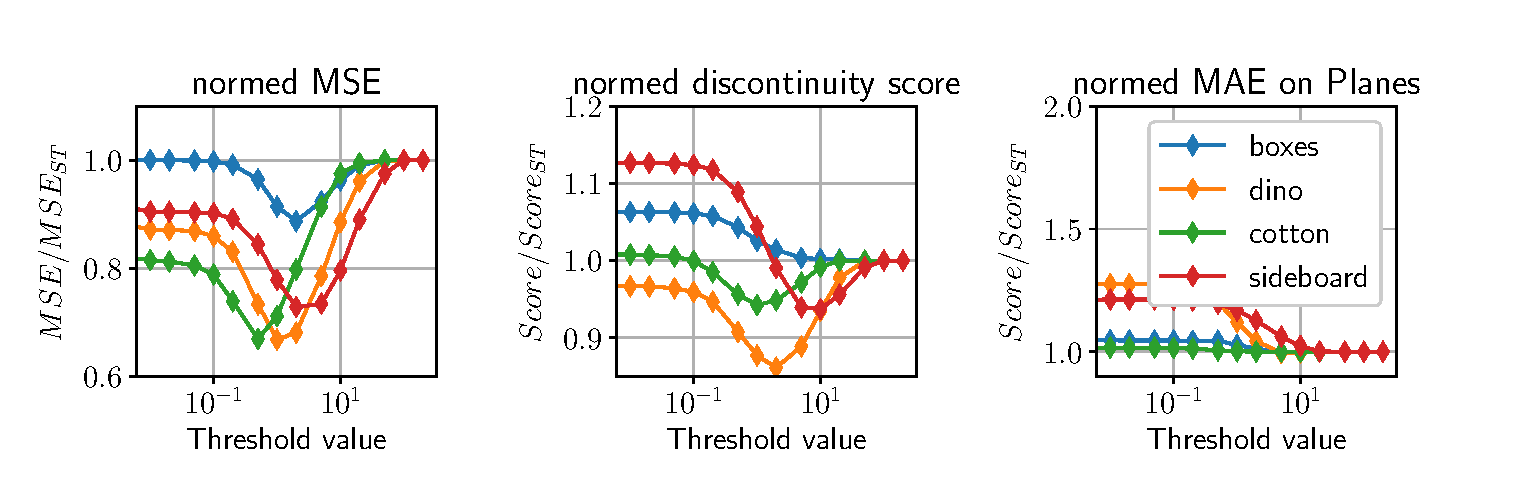
\includegraphics[width=1\linewidth]{images/thresh_params}
	\caption[Results when thresholding the Gradients in the EPI]{Results when thresholding the Gradients in the EPI are shown. All results are divided by the score obtained from the normal structure tensor algorithm. On the left the Mean Squared Error is shown, in the middle the discontinuity score is shown, on the right we see the Mean Average Error on planar surfaces in the scene. All metric scores follow the metrics from \cite{honauer2016benchmark}. }
	\label{fig:threshparams}
\end{figure}
\end{frame}

\begin{frame}
\frametitle{ Evaluation: Thresholding gradients}
\begin{figure}
	\centering
	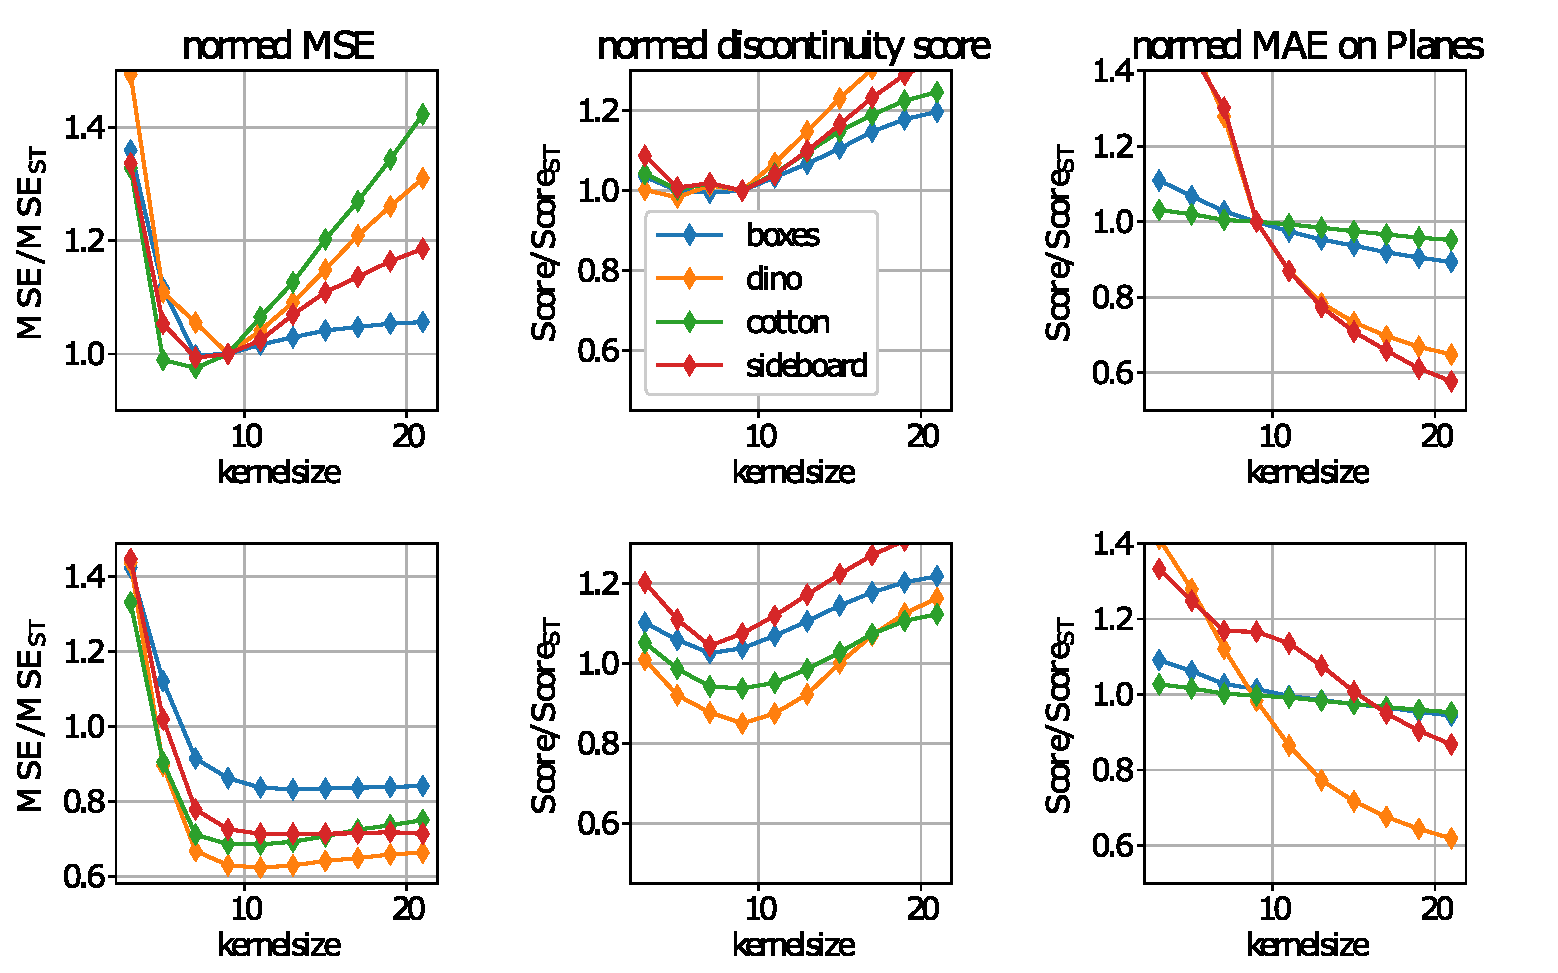
\includegraphics[width=1\linewidth]{images/old_outer}
	\caption[Varying kernelsize]{Varying the kernelsize, using the old ST pipeline (up) and with thresholded gradients (down)}
	\label{fig:oldouter}
\end{figure}
\end{frame}

\begin{frame}
\frametitle{Evaluation: Semiglobal Matching}
\begin{figure}
	\centering
	\includegraphics[width=1\linewidth]{images/sgm_params_contour_mse_100}
	\caption[mse_100]{Mean squared error for different (3) parameters}
	\label{fig:sgmparamscontourmse100}
\end{figure}
\end{frame}

\begin{frame}
	\frametitle{Evaluation:Table}
	\begin{table}
		\begin{tabular}{|c|c|c|c|c|c|}
			\hline 
			Method & Time(s)  & \multicolumn{4}{c|}{MSE} \\ 
			\hline 
			&  & boxes & cotton & dino & sideboard \\ 
			\hline
			Old Pipeline &\textbf{ 4.78} & 17.03 & 6.16 & 2.09 & 3.89 \\
			\hline 
			Sandclock & 6.81  & 18.55  & 6.78  & 2.23  & 4.14 \\ 
			\hline 
			epi-bilateralfilter &  43.96 &  19.26  & 6.41  & 2.22  & 4.16  \\ 
			\hline 
			bilateralfilter & 20.18  & 18.95  &  6.38 & 2.10  &4.32  \\ 
			\hline 
			Thresholding  & 6.06 & 15.57  & 4.38  & 1.39  & 3.03  \\ 
			\hline 
			occl. segm. & 11.28  & 18.08 &  3.39 & 1.78  & 3.91  \\ 
			\hline 
			altern. coh. +Treshold & 14.15  & 15.85  & 4.30  & 1.25  & 3.38  \\ 
			\hline 
			SGM& 8.90 & 14.98  & 3.84  & 1.75  & 3.18  \\ 
			\hline 
			SGM+Threshold & 12.75  & \textbf{13.31}  &\textbf{ 2.96}   &\textbf{ 1.11}   & \textbf{2.43} \\ 
			\hline 
			\hline
					\end{tabular} 
		\end{table}
	\end{frame}
\begin{frame}
\frametitle{Evaluation: Postprocessing}
\begin{table}
	\begin{tabular}{|c|c|c|c|c|c|}
		\hline 
		Method & Time(s)  & \multicolumn{4}{c|}{MSE} \\ 
		\hline 
		&  & boxes & cotton & dino & sideboard \\ 
		\hline
			pp Gauss 3 & & 12.59 & 4.80 & 1.68 & 2.92 \\
			\hline
			pp Gauss 5 & & 11.95 & 4.54 & 1.59 &  2.72 \\
			\hline 
			pp Gauss 7 & & 11.51 & 4.31 & 1.50 & 2.58 \\
			\hline
			pp Gauss 9 & &\textbf{ 11.34} & 4.16 & 1.46 & 2.52 \\
			\hline
			pp SGM & &12.0 & \textbf{2.15} &\textbf{ 1.08} & \textbf{1.98}\\
			\hline
			pp Median 3 & & 13.21 & 4.96 & 1.83 & 3.35 \\
			\hline
			pp Median 5 & & 12.73 & 4.76 & 1.76 & 3.20 \\
			\hline
		\end{tabular} 
	\end{table}
\end{frame}

\end{document}